% !TEX root = ../00_thesis.tex

% ------------------------------------------------------------------------------
\section{Synthesis of Compatible Multi-Mode Schedules}
\label{sec:multi_mode}
% ------------------------------------------------------------------------------


\TTW statically co-schedules all tasks and messages in order to satisfy tight deadline constraints~(\cref{sec:single_mode}).
To preserve a certain degree of adaptability at runtime, we support multiple operation modes.
Doing so requires to ensure predictable mode switches; that is, applications always meet their end-to-end deadlines~\objA and the persistent applications have compatible schedules in different modes~\objB.

% \TODO{needed?}
% We will formulate this schedule compatible with a continuity constraint~(\cref{def:continuity_constraint}). When the mode schedules are compatible, we say that the modes are \emph{conflict-free}.

The multi-mode case is essentially a multi-objective problem. One could decide to minimize the overall number of rounds used (\ie the sum of rounds in all the modes); however, it might also be interesting to optimize the ``most common mode''; this is, the mode in which the system operates most of the time.
Ultimately, one must weight the different modes to define a globally optimal solution.

\squarepar{%}
	Instead of solving the entire multi-mode problem at once, which would have scalability issues, we solve the problem sequentially: one mode at a time, in order of increasing priority.
	However, ensuring schedule compatibility between the different modes~\objective{2} creates dependencies, as illustrated below.%
}

\begin{example}
\label{exp:sched_conflict_basic}
	Let us consider the mode graph in \cref{fig:modeGraph} and assume that all applications are persistent.
	The modes are scheduled sequentially, starting with the highest-priority mode \mode{1}, which is freely scheduled.
	When mode \mode{2} is scheduled, the schedule for application \appl{2} is inherited from mode \mode{1}~\objective{2} and the schedules for applications \appl{3} and \appl{4} are synthesized without constraints.
	In \mode{3}, the specified applications, \appl{5} and \appl{6}, are new and can be scheduled without constraints.
	Then, in mode \mode{4}, the specified applications, \appl{1} and \appl{5}, have both been previously scheduled and thus must be inherited~\objective{2}.
	However, as mode \mode{3} has been scheduled without constraint, the schedule synthesized for \appl{5} may be non-compatible with that of \appl{1} from mode \mode{1}. This leads to a conflict in \mode{4} and thus renders the sequential synthesis of the multi-mode problem unfeasible~(illustrated in \cref{fig:example_sched}).
\end{example}

\begin{figure}
\centering
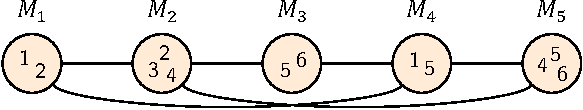
\includegraphics[scale=1]{modeGraph}
\caption{The mode graph \modeGraph discussed in \cref{exp:sched_conflict_basic,exp:sched_domain}.
\capt{Five modes are represented by circles, the possible transitions between modes as arcs. Six applications \appl{1} to \appl{6} are specified. The specification is shown with the numbers in the circles; \eg $S_1 = \{\appl{1},\appl{2}\}$. Mode \modei has priority $i$.}}
\label{fig:modeGraph}
\end{figure}

\begin{figure}
	\begin{subfigure}[t]{.48\linewidth}
		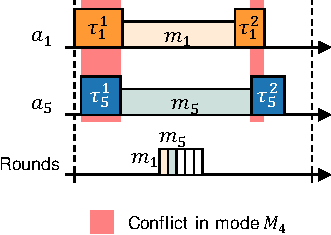
\includegraphics[scale=1]{example_sched_conflict}
		\caption{%
		\appl{5} is scheduled in mode \mode{3} without considering the previously computed schedule of \appl{1}, which leads to a conflict in mode \mode{4}.}
		\label{subfig:example_sched_conflict}
	\end{subfigure}%
	\hfill
	\begin{subfigure}[t]{.48\linewidth}
		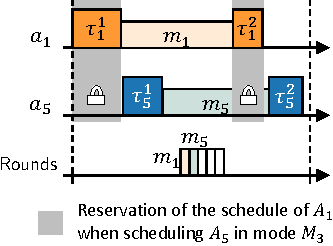
\includegraphics[scale=1]{example_sched_reservation}
		\caption{%
		\appl{5} is scheduled in mode \mode{3} considering the schedule of \appl{1} as \emph{reserved}. Thus, a compatible schedule for \appl{5} is computed, which prevents conflicts due to schedule inheritance in mode \mode{4}.}
		\label{subfig:example_sched_reservation}
	\end{subfigure}
	\caption{%
		Representations of the schedule of applications \appl{1} and \appl{5} from~\cref{exp:sched_conflict_basic}.
		For the sake of illustration, we consider that all tasks are mapped to the same node.
		\appl{1} and \appl{5} are scheduled respectively in mode \mode{1} and \mode{3}, and must both be inherited in mode \mode{4}.
		In~\cref{subfig:example_sched_conflict}, overlapping task schedules result in a conflict, while in~\cref{subfig:example_sched_reservation}, it was prevented by reserving \appl{1}'s schedule.
		The situation is different for the messages: overlapping message schedules is no issue, it simply represents a time interval where both messages can be served during the same round, as shown in this example.
	}
	\label{fig:example_sched}
\end{figure}

As illustrated in~\cref{exp:sched_conflict_basic}, it may be necessary to ``reserve the space'' of previously scheduled applications (\ie in previous modes) in order to avoid schedule conflicts.
The simplest approach is to reserve the space of \emph{all previous scheduled applications}. This is definitely safe but often pessimistic, as there may not be risk of conflicts for certain applications.

In this section, we derive the set of schedule reservations that is necessary and sufficient to prevent inheritance conflicts.
We first formalize the continuity constraints that we want to satisfy~\objB~(\cref{subsec:continuity_constraints}).
Then, we characterize conflicting modes and formalize how continuity constraints may lead to conflicts~(\cref{subsec:conflict_def}).
Finally, we derive the minimally restrictive reservations that are necessary and sufficient to prevent conflicts while satisfying \objB~(\cref{subsec:min_constraints}).

% ------------------------------------------------------------------------------
%	a.	Application domain decomposition -> Real-time apps to be preserved across diff modes
\subsection{Continuity Constraints}
\label{subsec:continuity_constraints}

The schedule synthesis returns the application schedules, \ie the task and message offsets and the message deadlines; and the round schedules, \ie the round starting times and the allocation vector.
We abstract an application schedule with a scheduling function $s$ as follows.

\begin{definition}[Scheduling function]
\label{def:sched_funtion}
The scheduling function $s$ is defined over the set of applications \appset and returns, for a given application \app, all the parameters characterizing the schedule of application \app. The schedule of an application \app is denoted by $s(\app)$.
The scheduling function is extended to sets of applications as follows.
\begin{equation*}
\forall \, S \subset \appset \; , \quad s(S) = \bigcup_{\app\in S} s(\app)
\end{equation*}
$s_\mode{}(\app)$ denotes the schedule of application \app in mode \modeany.
\end{definition}

All persistent applications $\app \in \persappset$ are subject to continuity constraints,  formalized as follows.
\begin{definition}[Continuity constraint]
\label{def:continuity_constraint}
\begin{align}
\intertext{$\forall\, \app \in \persappset, \; \forall\, (\modei, \modej) \in \modeset^2,$}
& \app \in \modei \; \wedge \; \app \in \modej \; \wedge \; \modeGraph(\modei,\modej) = 1
	\quad \Rightarrow \quad
	s_\modei(\app) = s_\modej(\app)
\end{align}
In other words, an executing application must keep the same schedule, regardless of mode changes.
\end{definition}


\begin{definition}[Schedule domains]
\label{def:sched_domains}
The schedule domains of an application are the (possibly multiple) subsets of modes in which the application schedule must remain the same.
\end{definition}

\begin{corollary}
	%Non real-time applications have schedule domains of size 1.
	Two modes \modei and \modej belong to the same schedule domain of an application $\app \in \persappset$ if and only if
	\begin{itemize}
		% \item $\app \in \persappset$,
		\item \app is scheduled in both modes, \ie $\app \in \modei \; \wedge \; \app \in \modej$, and
		\item There is a possible transition between the two modes, \ie $\modeGraph(\modei, \modej) = 1$.
	\end{itemize}
\end{corollary}

\proof
Multiple modes belong to the same schedule domain because of a continuity constraint.
The formalization of the schedule domains directly follows from~\cref{def:continuity_constraint}
\qed

The mode graph can be analyzed to extract the schedule domains of any application.
A simple approach entails considering the sub-graph \modeGraphA from \modeGraph, \ie where one keeps only the modes in which application \app is specified.
Every connected component of \modeGraphA is a schedule domain of \app.

\begin{hypothesis}
	\label{hyp:single_domain}
	We consider in the rest of this chapter that (i)~all applications are persistent, and (ii)~applications have a single scheduling domain.
\end{hypothesis}

\cref{hyp:single_domain} induces no loss of generality. Indeed, non-persistent applications present in multiple modes can be replaced by distinct applications, with the same parameters, executing in one mode each.
Similarly, persistent applications different scheduling domains can be replicated into different applications having one domain each.
This is illustrated in the following example.

\begin{example}\label{exp:sched_domain}
Consider again the mode graph in \cref{fig:modeGraph}. Application \appl{6} has two distinct application domains, $\{\mode{3}\}$ and $\{\mode{5}\}$, which can be modeled as two distinct applications \appl{6.3} and \appl{6.6} executing in \mode{3} and \mode{6} respectively.

On the contrary, \appl{1} has only one schedule domain, $\{\mode{1},\mode{4}\}$.
If \appl{1} is not persistent, the continuity constraint does not apply~(\cref{def:continuity_constraint}).
Thus, \appl{1} can be equivalently modeled as two distinct applications \appl{1.1} and \appl{1.4} executing in \mode{1} and \mode{4} respectively.
\end{example}


% ------------------------------------------------------------------------------
\subsection{Characterization of Conflicts}
\label{subsec:conflict_def}

\squarepar{%}
	As illustrated in \cref{exp:sched_conflict_basic}, the continuity constraint may lead to conflicts, leading to the failure of the multi-mode schedule synthesis problem, while a solution could exist.
	In particular, if a given mode \mode{} belongs to the schedule domains of two different applications which have been independently scheduled in higher priority modes, there is a risk of conflict, \ie the two inherited schedules may be non-compatible.
	This section formalizes the notions of (virtual) legacies and conflicting modes.
	$\overline{X}$ denotes the complement of $X$; \ie $\overline{X} = \appset \setminus X$.
	For each mode \modei, we define four sets of applications.%
}

\textbf{Known applications} are the applications previously scheduled in higher priority modes. The set of known applications of mode \modei is denoted \knownAppi:
	\begin{equation}
	\knownAppi = \cup_{j = 1}^{i-1} \; \modej
	\end{equation}

\textbf{Free applications} are the newly scheduled applications in mode \modei, \ie no higher priority mode belongs to the schedule domain of these applications.
	The set of free applications of mode \modei is denoted \freeAppi :
	\begin{equation}
	\freeAppi = \modei \; \cap \; (\appset \setminus \knownAppi) = \modei \; \cap \; \overline{\knownAppi}
	\end{equation}

\textbf{Legacy applications} are the applications previously scheduled in higher priority modes which must be scheduled in mode \modei.
	Since we assume a single scheduling domain~(\cref{hyp:single_domain}), \modei necessarily belongs to the same schedule domain as these higher priority modes and the legacy application schedules must be inherited.
	The set of legacy applications of mode \modei is denoted \legAppi:
	\begin{equation}
	\legAppi = \modei \; \cap \; {\knownAppi}
	\end{equation}

Finally, \textbf{virtual legacy applications} are the applications previously scheduled in higher priority modes which are not scheduled in mode \modei.
	The set of virtual legacy applications of mode \modei is denoted \virtlegAppi:
	\begin{equation}
	\virtlegAppi = (\appset \setminus \modei)\; \cap \; {\knownAppi} = \overline{\modei} \; \cap \; {\knownAppi}
	\end{equation}
The virtual legacy applications of \modei are not executed in \modei; they simply have been scheduled in higher-priority modes. As illustrated in \cref{exp:sched_conflict_basic}, it may be necessary to ``reserve the space'' of some of these virtual legacy applications in order to avoid future inheritance conflicts.


The schedule of two applications \appA and \appB are said in conflict when two tasks from \appA and \appB respectively are mapped to the same node and are scheduled during overlapping time intervals.
We denote by $s(\appA) \cap s(\appB) \not= \emptyset$ the property that ``\appA and \appB are in conflict''.
%
% As illustrated by Example~\ref{exp:sched_conflict_basic}, a conflict occurs when the legacy applications of one mode have non-compatible schedules.
%are not conflict-free, \ie the inherited schedules of legacy applications are overlapping.

\begin{definition}[Conflict-free]
A set of applications $S$ is said to be conflict-free when there is no conflict between the schedules of the applications in $S$. We denote by \cf{S} the property that $S$ is conflict-free, and $\overline{\cf{S}}$ denotes that the set $S$ is in conflict.
Formally,
\begin{equation*}
\cf{S} \quad \Leftrightarrow  \quad \bigcap_{A \in S} \; s(A) = \emptyset
\end{equation*}
A mode is said to be conflict-free if its legacy applications are conflict-free. In other words, $\forall \modei \in \modeset$,
\begin{equation*}
\cf{\modei} \quad \Leftrightarrow  \quad \cf{\legAppi}
\end{equation*}
% a mode \modei is conflict-free if and only if \cf{\legAppi}.
The schedule \sched{\modei} of mode \modei is valid only if $\cf{\modei}$.
\end{definition}

\begin{corollary}
\label{cor:nec_precond}
	A valid schedule for a mode $\modei \in \modeset$ can only exist if the virtual legacy applications of \modei are conflict-free; that is,
	\begin{equation*}
	\cf{\legApp{i}} \; \Leftarrow \; \text{``Sched(\modei) is feasible''}
	\end{equation*}
	% A necessary precondition for the schedule synthesis of any mode \modei to be feasible is that \modei is conflict-free, \ie $$.
\end{corollary}

\proof Using~\cref{exp:sched_conflict_basic} as a counter-example, $\overline{\cf{\legApp{4}}}$ makes it impossible to derive a valid schedule for \mode{4}.
\qed




% ------------------------------------------------------------------------------
\subsection{Minimal Inheritance Constraints}
\label{subsec:min_constraints}

The single-mode schedule synthesis algorithm~(\cref{alg:outerlayer}) is complete: if the problem is feasible, a valid schedule is found. In particular, the scheduled mode is conflict-free; \ie \cf{\modei}.
Certain applications are subject to continuity constraints~(\cref{subsec:continuity_constraints}), which are satisfied by fixing the schedules of legacy applications \legAppi in the MILP formulation for \modei.
However, this can lead to a feasible schedule only if \cf{\legAppi}~(\cref{cor:nec_precond}).

\cref{exp:sched_conflict_basic} illustrated that inheriting legacy applications is not sufficient to prevent conflicts.
Thus, we now derive the subset of the virtual legacy applications \virtlegAppi of a \modei that is necessary and sufficient to reserve in order to guarantee the absence of conflict due to continuity constraints.
In other words, the objective is that for any mode \modei,
\begin{align}\label{eq:obj_conflict-free}
&\forall \, k \in [1..i-1], \; \text{``\sched{\mode{k}} is feasible''} \quad \Rightarrow \quad \cf{\legApp{i}}
\end{align}

% Our approach uses the concept of virtual legacy applications to \emph{reserve the space} of inherited application schedules from higher-priority modes to enforce \eqref{eq:obj_conflict-free}, \ie to guarantee that legacy application inheritance does not induce conflicts in lower-priority modes.

%1. Redefinition of the \sched function, with the let and virtual leg as constraints
First, we formalize the constraints on the \sched{} function such that continuity constraints are enforced and conflicts are prevented.
% \begin{align}
% \label{eq:sched_redef}
% \begin{tabular}[t]{@{}l@{\;}l@{\;}l}
% $Sched: \; \modeset \;
% 	\longmapsto \; \sched{M}$
% 	&
% 	s.t.
% 	& $\cf{\modei}$\\
% &&$\forall\, \app \in \legApp{i} \cap S_{j}, \, j < i, \;
% 			s_\modei(\app) = s_\modej(\app)$\\
% &&$\forall\, \app \in \freeAppi, \; s(\app) \; \cap \; s(\minvirtlegApp{i}{A}) = \emptyset$
% 	\end{tabular}
% \end{align}
\begin{align}
\label{eq:sched_redef}
Sched: \; &\modeset \; \longmapsto \; \sched{M}\\
\nonumber
s.t. \quad
		& \cf{\modei}\\
\nonumber
		& \forall\, \app \in \legApp{i} \cap \modej, \, j < i, \;	s_\modei(\app) = s_\modej(\app)\\
\nonumber
		& \forall\, \app \in \freeAppi, \; s(\app) \; \cap \; s(\minvirtlegApp{i}{\app}) = \emptyset
\end{align}

\squarepar{%}
	In \cref{eq:sched_redef}, the first constraint \cf{\modei} is necessary for the schedule to be valid. The second enforces the continuity constraints of applications. Finally the third constraint aims to enforce \cref{eq:obj_conflict-free}. The idea is that the newly scheduled application in mode \modei, \ie \app $\in$ \freeAppi, should be compatible with the schedules of some virtual legacies. The objective is to derive the minimal sets \minvirtlegApp{i}{\app} for any $\app \in \freeAppi$ such that condition \cref{eq:obj_conflict-free} is satisfied.%
}

\begin{theorem}[Minimal virtual legacy sets]
\label{thm:minVirtLegacy}
For any mode \modei and any application \app in \freeAppi, the minimal set of virtual legacy applications \minvirtlegApp{i}{\app} necessary and sufficient to satisfy \eqref{eq:obj_conflict-free} is given by
\begin{equation}\label{eq:minVirtLegSets}
\minvirtlegApp{i}{\app} = \{ \appX \in \virtlegAppi \; |\;  \exists\, j>i, \quad \app \in  \legAppj \;\; \wedge \;\; \appX \in \legAppj \}
\end{equation}
\end{theorem}

%%%%%%%%%%%%%%%%%%%%%%%%%%%%%%%%%%%%%%%%%%%%%
%% Theorem proof
%%%%%%%%%%%%%%%%%%%%%%%%%%%%%%%%%%%%%%%%%%%%%
\proof
We first prove that virtual legacy sets as defined in \eqref{eq:minVirtLegSets} are sufficient to satisfy \eqref{eq:obj_conflict-free}. This is done by recurrence.

For the highest priority mode \mode{1}, by definition, $\legApp{1} = \emptyset$, thus \cf{\legApp{1}}.
Let us assume that for any $k \in [1 .. i]$,
\sched{\mode{k}} is feasible in the sense of \eqref{eq:sched_redef}. This induces that \cf{S_k}, hence \cf{\legApp{k}} for any $k \in [1 .. i]$.
Let us finally assume that \legApp{i+1} is \emph{not} conflict-free; that is,
\begin{equation}\label{eq:hyp_rec_conflict}
	\overline{\cf{\legApp{i+1}}}  \quad \Leftrightarrow  \quad \bigcap_{A \in \legApp{i+1}} \; s(A) \not= \emptyset
\end{equation}
Therefore,
\begin{align}
\label{eq:square}
\eqref{eq:hyp_rec_conflict} \quad &
	\Rightarrow \quad \exists \, (A,B) \in \legApp{i+1}^2, \; s(A) \cap s(B) \not= \emptyset \\
\label{eq:square2}
	&
	\Rightarrow \quad
		\left\lbrace
		\begin{tabular}{@{\,}l@{\;\;}l@{\;\;}l}
		$\exists ! \, \mode{a}, \;A \in \freeApp{a} $&$\wedge $&$ a < i+1$ \\
		$\exists ! \, \mode{b}, \;B \in \freeApp{b} $&$\wedge $&$ b < i+1$ \\
		\end{tabular}
		\right.
\intertext{where $\exists !$ means ``there exists a unique''.
Without loss of generality, we consider $a\leq b$. If $a=b$, then $S_a = S_b$ and $\cf{S_a} \equiv \cf{S_{b}}$. Therefore,}
	& \phantom{\Rightarrow} \quad
		\bigcap_{A \, \in\,  S_a = S_b} \; s(A) = \emptyset \quad \text{in particular}\\
	& \Rightarrow \quad
		s(A) \cap s(B) = \emptyset \quad \text{which contradicts \eqref{eq:square}}\\
	& \Rightarrow \quad
		a < b
\end{align}
In other words, mode \mode{a} has higher priority than mode \mode{b}. Therefore, \app belongs either to \legApp{b} or \virtlegApp{b} by definition of those sets.
By hypothesis, \cf{S_{b}} and \eqref{eq:square2} : $B \in \freeApp{b}$, thus
\begin{equation*}
A \in \legApp{b} \quad \Rightarrow \quad s(A) \cap s(B) = \emptyset
\end{equation*}
which contradicts \eqref{eq:square}. Hence necessarily,
$A \in \virtlegApp{b}$. Furthermore,
\begin{equation}
\left.
	\begin{tabular}{@{}l}
	$\eqref{eq:square2} : i+1 > b$\\
	$\eqref{eq:square} : A \in \legApp{i+1}$\\%
	$\eqref{eq:square} : B \in \legApp{i+1}$
%	$\left.%
%		\begin{tabular}{@{}l@{\;}l}
%		$\eqref{eq:square2} :$&$ B \in \freeApp{b}$\\
%		$\eqref{eq:square}  :$&$ B \in \legApp{i+1}$\\
%		\end{tabular}
%	\right\rbrace
%	\; \Rightarrow \; \freeApp{b} \cap \legApp{i+1} \not= \emptyset$
	\end{tabular}
\right\rbrace
\; \text{Taking }b=i\text{ and }j = i+1, \quad \eqref{eq:minVirtLegSets}\; : \;
%{\Rightarrow} \;
A \in \minvirtlegApp{b}{B}
\end{equation}

\squarepar{%}
	By hypothesis, \sched{\mode{b}} is feasible, thus $s(\appB) \; \cap \; s(\minvirtlegApp{b}{B}) = \emptyset$, which yields $s(B) \cap s(A) = \emptyset$ and contradicts \eqref{eq:square} again.
	Therefore, the recurrence hypothesis is necessarily false.
	Hence, if for any $k \in [1 .. i]$, \sched{\mode{k}} is feasible in the sense of \eqref{eq:sched_redef}, then \cf{\legApp{i+1}}.
	By recurrence, we can conclude that the \emph{virtual legacy sets as defined by \eqref{eq:minVirtLegSets} are sufficient} to satisfy \eqref{eq:obj_conflict-free}.%
}

We now prove they are also necessary.
Let us consider smaller virtual legacy sets than defined by \eqref{eq:minVirtLegSets}, \ie $\exists \; i \in [1..M],\, \app \in \freeAppi, \;\;\minminvirtlegApp{i}{A} \nsubseteq \minvirtlegApp{i}{A}$. Let us further assume that \sched{} is redefined to replace \minvirtlegApp{}{} by \minminvirtlegApp{}{}. By hypothesis,
\begin{equation}
\label{eq:nec_cond1}
\exists \; \appX \in \appset, \; \appX \in \minvirtlegApp{i}{A}\; \wedge \; {\appX \notin \minminvirtlegApp{i}{A}}
\end{equation}
Furthermore,
\begin{align}
\label{eq:nec_cond4}
\appX \in \minvirtlegApp{i}{A}
	&\quad \Rightarrow \quad
	\appX \in \virtlegApp{i} \quad \Rightarrow \quad {\appX \notin S_{i}}\\
\label{eq:nec_cond2}
\appX \in \minvirtlegApp{i}{A}
	&\quad \Rightarrow \quad
	\exists \; j>i, \quad {\app \in \legApp{j}} \; \wedge \; \appX \in \legApp{j}
%\label{eq:nec_cond3}
%\freeApp{i} \cap \legApp{j} \not= \emptyset
%	&\quad \Rightarrow \quad
%	\exists \; \dashuline{B \in \freeApp{i}}, \quad \underline{B \in \legApp{j}}
\end{align}
Assuming that \sched{\modei} is feasible, the resulting schedule guarantees that
\begin{equation}
\label{eq:nec_cond5}
\begin{tabular}{l@{\quad\quad}cp{30pt}}
	&
	\cf{\modei}
	&\\[5pt]
\texttt{and}
	&
	$\forall \, \app \in \freeApp{i},\; s(\app) \, \cap \, s(\minminvirtlegApp{i}{A}) = \emptyset$
	&
\end{tabular}
\end{equation}
However, \eqref{eq:nec_cond1} : $\appX \notin \minminvirtlegApp{i}{A}$ and \eqref{eq:nec_cond4} : $\appX \notin S_{i}$. Hence the schedule $s(\app)$ may be synthesized such that $s(A) \cap s(X) \not= \emptyset$. According to \eqref{eq:nec_cond2} : $(A,X) \in \legApp{j}^2$, thus this induces a conflict in mode \modej.
Hence, we can conclude that no sets \minminvirtlegApp{}{} smaller that \minvirtlegApp{}{} are sufficient to satisfy \eqref{eq:obj_conflict-free}.

Therefore, one concludes that the virtual legacy sets \minvirtlegApp{}{} as defined in \eqref{eq:minVirtLegSets} are both necessary and sufficient for the schedule synthesis method to satisfy \eqref{eq:obj_conflict-free}, \ie to guarantee that legacy applications schedule inheritance does not lead to conflicts in lower-priority modes.
In other words, \minvirtlegApp{}{} from \eqref{eq:minVirtLegSets} define the \emph{minimally restrictive constraints sets} such that \sched{} as defined in \eqref{eq:sched_redef} satisfies \eqref{eq:obj_conflict-free}.
\qed
